\chapter{Clustering Algorithms}
\label{sec:clustering_algorithms}
In the application CPlan the street network is generated as a graph as described in \ref{CPlan}. To separate and select areas with specific characteristics the networks have been analysed by machine learning clustering algorithms. In this section the different clustering algorithms are analysed and the generated results produced by our implementations in CPlan are compared.

\section{K-Means}  \label{sec:K-Means}
\subsection{Description}
The K-Means algorithm detects the clusters / partitions by measuring the euclidean distance between the cluster centroids and the position of the street junctions. The algorithm uses the following approach:

\begin{enumerate}
    \item A number of points are inserted into the graph and used as centroids.
    \item All graph points are assigned to their nearest centroids.
    \item The centroids are moved to the center of their assigned graph points.
    \item Until the maximum number of iterations is reached this process is repeated starting by loop item 2.
\end{enumerate}
Because the K-Means algorithm can find local minima, this process needs to be executed more than once. The result with the best found solution will be selected.

\subsection{Implementation}
The added implementation in CPlan\citep{cPlan:2015} is an optimised K-Means version based on the paper \textit{An Efficient k-Means Clustering Algorithm: Analysis and Implementation} \cite{kmeans:2002} with a runtime of $O(n\ insert\ here)$
%TODO Kmenas++ inteligent start points not k-d-tree
\subsection{Speed Optimization}
The ETH-Zurich provided the following networks: Bad Berka (552 nodes, 626 edges), Weimar (2012 nodes, 2646 edges) and Zurich (27446 nodes, 35121 edges). The network Zurich with factor 13 more edges than Weimar resulted in long processing time. A speed improvement can be achieved by running the K-Means iterations in parallel. Every iteration can be executed free of side effects. The measurements and comparisons of the results are provided in the section Practical Task/Measurements \ref{sec:measurements};

\subsection{Result}
The implementation in CPlan \ref{CPlan} produced the following image \ref{fig:KmeansGenerated} based on the city of Weimar. All streets in one cluster are marked with the same colour, the transitions between clusters are marked black.
\begin{figure}[!h]
    \centering
    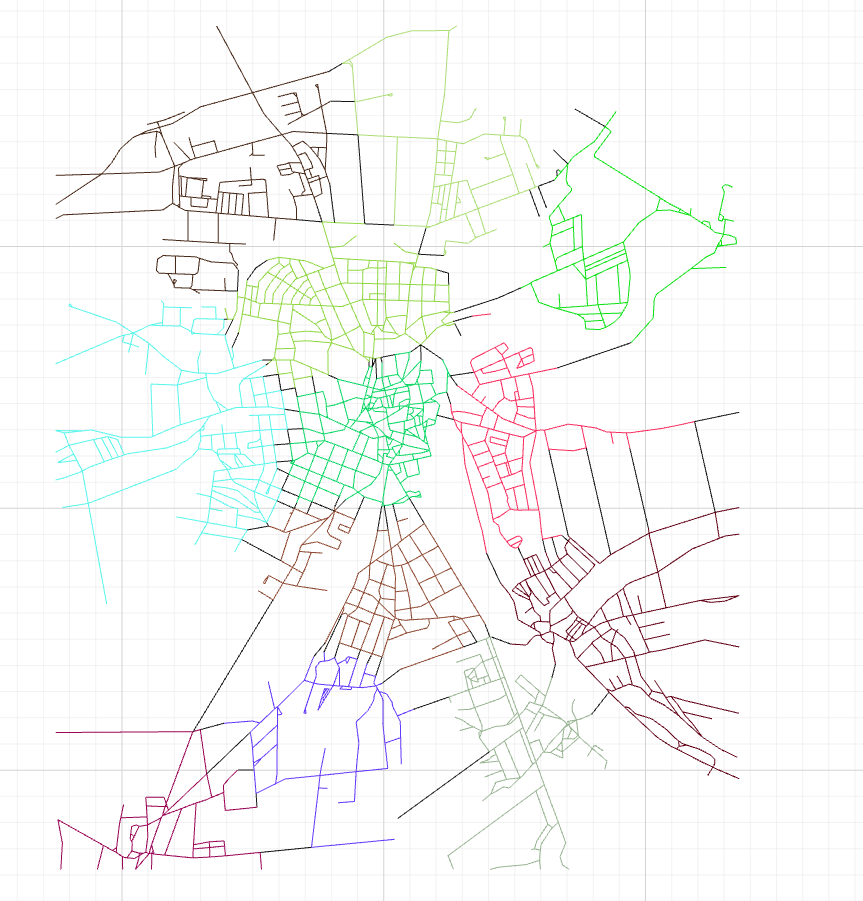
\includegraphics[width=\textwidth]{clusteranalysis_kmeans_result.png}
    \caption{K-Means cluster analysis of Weimar\label{fig:KmeansGenerated}}
\end{figure}

\subsection{Problem} \label{sec:kmenasProblem}
The algorithm is based on the euclidean distance between cluster centroids and street junctions, the edge data (e.g. street length) is not used. As a result it leads to unexpected transitions between clusters. In the image \ref{fig:KmeansProblem} the result can be seen in the read circle where only one point is marked as outer cluster. The two black lines represent the cluster transitions.
\begin{figure}[!h]
    \centering
    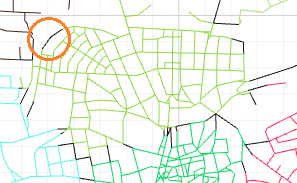
\includegraphics[width=0.6\textwidth]{clusteranalysis_kmeans_problem.png}
    \caption{Problem of K-Means clustering\label{fig:KmeansProblem}}
\end{figure}

\subsection{K-Means with Shortest Path} \label{sec:K-Means_shortest_path}
To solve the problem of unexpected transitions between clusters the best result of the K-Means algorithm can be combined with the distance measurement of a shortest path algorithm (Dijkstra / FloydWarshall). These algorithms are used by hierarchical clustering \ref{sec:shortest_path}. The edges are assigned by the edge data (e.g. street length) to the nearest cluster. Therefore the result is a connected graph. This means every vertex can be reached from every other vertex within a cluster. In the generated figure \ref{fig:Kmeansshortestp} the artefacts described in \ref{kmenasProblem} are removed.

Additional calculation time is needed for the shortest path algorithm. The differences can be compared in the section Practical Task/Measurements \ref{sec:measurements};

\begin{figure}[!h]
    \centering
    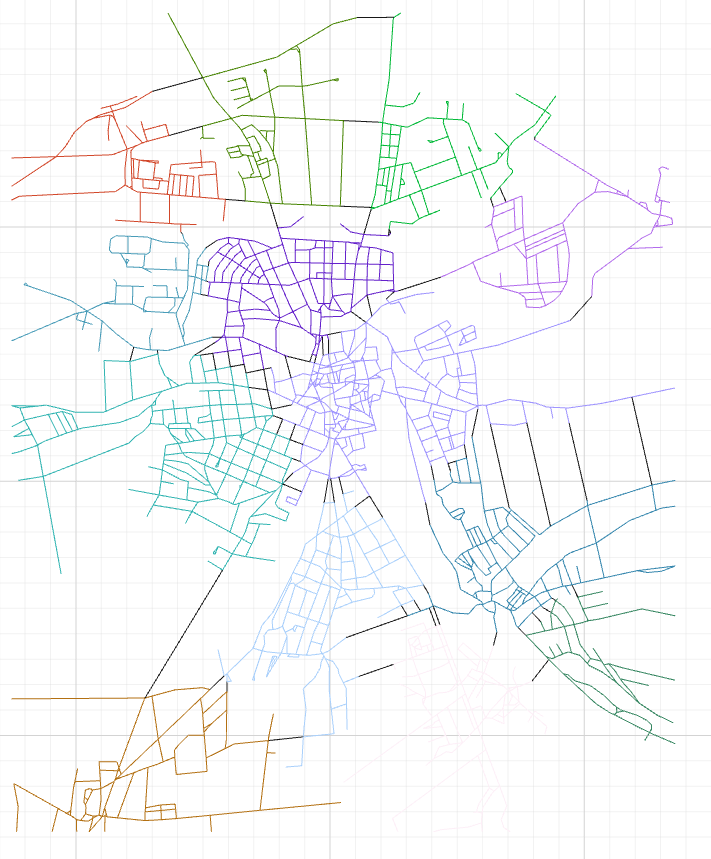
\includegraphics[width=0.9\textwidth]{clusteranalysis_kmeansExt_result.png}
    \caption{K-Means clustering with shortest path\label{fig:Kmeansshortestp}}
\end{figure}
